% !TEX program = latexmk
% !TEX options = -synctex=1 -interaction=nonstopmode -file-line-error
%% Презентация ВКР (Beamer, pdflatex, T2A).
%% Содержание и формулировки соответствуют тексту ВКР; используются все
%% изображения из ../images.
%%
%% Автосборка: в Cursor/VS Code с LaTeX Workshop при сохранении или
%% изменении зависимостей (см. .vscode/settings.json). Либо в терминале:
%%   make watch-presentation

\documentclass[aspectratio=169,12pt]{beamer}

%% --- Локализация и шрифты, совместимые с pdflatex ------------------------
\usepackage{cmap}
\usepackage[T2A]{fontenc}
\usepackage[utf8]{inputenc}
\usepackage[english,russian]{babel}
\usepackage{mathptmx}                 % Times-подобный основной шрифт
\usepackage{amsmath,amssymb,mathtools}
\usepackage{icomma}
\usepackage{graphicx}
\usepackage{booktabs}
\usepackage{array}
\usepackage{tabularx}
\usepackage{caption}
\usepackage{xcolor}
\usepackage{gensymb}

%% --- Тема и цветовая схема ----------------------------------------------
\usetheme{Madrid}
\usecolortheme{seahorse}
\useinnertheme{rectangles}
\useoutertheme{infolines}
\setbeamertemplate{navigation symbols}{}
\setbeamertemplate{caption}[numbered]
\captionsetup{labelformat=empty,labelsep=none,font=footnotesize}

\definecolor{itmoblue}{RGB}{0, 102, 153}
\setbeamercolor{structure}{fg=itmoblue}
\setbeamercolor{frametitle}{fg=white,bg=itmoblue}
\setbeamercolor{title}{fg=itmoblue}
\setbeamercolor{section in head/foot}{bg=itmoblue,fg=white}
\setbeamercolor{author in head/foot}{bg=itmoblue!90,fg=white}
\setbeamercolor{title in head/foot}{bg=itmoblue!70,fg=white}
\setbeamercolor{date in head/foot}{bg=itmoblue!90,fg=white}

\setbeamerfont{frametitle}{size=\large,series=\bfseries}
\setbeamerfont{title}{size=\Large,series=\bfseries}

%% --- Пути к рисункам -----------------------------------------------------
\graphicspath{{../images/}{images/}}

%% --- Метаданные ----------------------------------------------------------
\title[Сопровождение пользователя на омни-роботе]{%
Разработка алгоритма управления мобильным роботом\\
в условиях квартиры с динамически изменяющейся обстановкой}
\author[Н.\,И.\,Кудрявцев]{%
Кудрявцев Никита Игоревич \\[0.3em]
{\small Научный руководитель: Перегудин Алексей Алексеевич}}
\institute[Университет ИТМО]{%
Университет ИТМО\\
Факультет систем управления и робототехники\\
Направление: Робототехника и искусственный интеллект\\
Образовательная программа: Мехатроника и робототехника}
\date{Санкт-Петербург, \the\year}

\begin{document}

%% =========================================================================
\begin{frame}[plain]
    \titlepage
\end{frame}

%% --- Содержание ---------------------------------------------------------
\begin{frame}{Содержание}
    \tableofcontents
\end{frame}

%% =========================================================================
\section{Постановка задачи}

\begin{frame}{Актуальность и предмет работы}
    \textbf{Сценарий.} Сервисный мобильный робот в типовой квартире:
    автономное сопровождение подвижного пользователя при наличии
    динамических препятствий.
    \medskip

    \textbf{Сложность.} Одновременная формализация разнородных
    требований:
    \begin{itemize}
        \item удержание целевой дистанции и центрирование цели в
              кадре камеры;
        \item обход статических и подвижных препятствий;
        \item плавность управления;
        \item корректное поведение при потере наблюдаемости цели.
    \end{itemize}
    \medskip

    \textbf{Подход.} Стохастическая реализация модельного
    прогнозирующего управления (MPPI) в составе навигационного стека
    ROS\,2 / Nav2 с пользовательскими критиками траектории.
\end{frame}

\begin{frame}{Цель и задачи}
    \textbf{Цель.} Разработка и экспериментальное исследование
    программного обеспечения автономного мобильного омни-робота для
    задачи сопровождения пользователя в квартирной среде с
    динамическими препятствиями на базе MPPI.
    \medskip

    \textbf{Задачи.}
    \begin{enumerate}
        \item Анализ подходов к локальному планированию (DWA, MPC,
              MPPI) и SLAM, обоснование выбора.
        \item Кинематическая модель омни-платформы Mecanum и
              формализация составной функции потерь.
        \item Воспроизводимая контейнерная среда (Docker, ROS\,2,
              Gazebo).
        \item Модель робота, узлы восприятия и моста навигационных
              целей.
        \item Пользовательские критики MPPI: \texttt{TargetCameraCritic}
              и \texttt{PotentialFieldCritic}.
        \item Серия экспериментов и количественная оценка решения.
    \end{enumerate}
\end{frame}

%% =========================================================================
\section{Обзор и обоснование подхода}

\begin{frame}{Сравнение методов локального планирования}
    \footnotesize
    \begin{tabularx}{\textwidth}{l X X X}
        \toprule
        & \textbf{Реактивные (DWA, потенц.\ поля)}
        & \textbf{Классический MPC}
        & \textbf{MPPI} \\
        \midrule
        Разнородные требования
        & ограниченно (эвристика)
        & да (гладкие штрафы)
        & да (произвольные штрафы) \\
        Негладкие штрафы / costmap
        & ограниченно
        & нет
        & \textbf{да} \\
        Параллелизм по сэмплам
        & ---
        & ---
        & \textbf{да} \\
        Локальные минимумы
        & уязвим
        & уязвим
        & устойчив (стохастика) \\
        \bottomrule
    \end{tabularx}
    \medskip

    \textbf{Выбор:} MPPI как локальный контроллер, \texttt{slam\_toolbox} для
    SLAM, \textbf{Nav2} как навигационный стек.
\end{frame}

%% =========================================================================
\section{Модель платформы}

\begin{frame}{Кинематическая схема омни-платформы Mecanum}
    \begin{columns}[T,onlytextwidth]
        \column{0.46\textwidth}
        \begin{figure}
            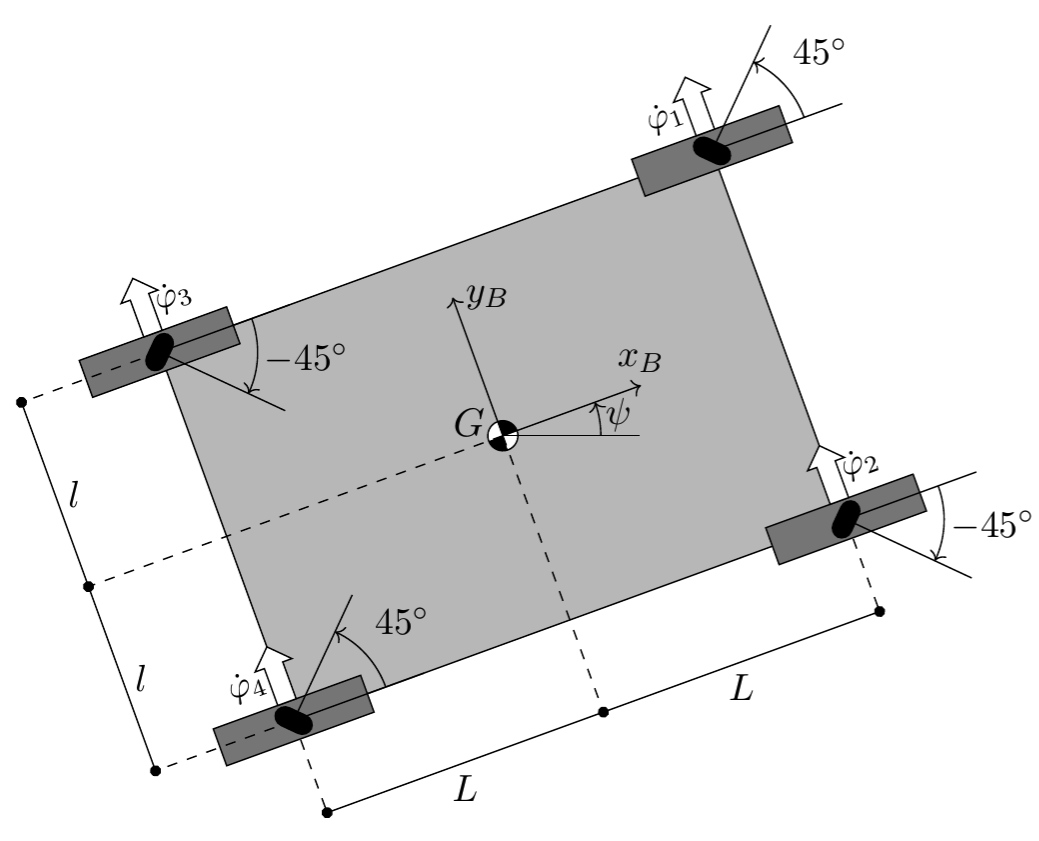
\includegraphics[width=\linewidth]{omni_scheme.png}
            \caption{Кинематическая схема омни-платформы}
        \end{figure}
        \column{0.54\textwidth}
        Связь скоростей корпуса и глобальных координат:
        \[
        \dot{\mathbf{x}} = R(\psi)\,\mathbf{u},\quad
        \mathbf{u} = [v_x,\,v_y,\,\omega]^{\top}.
        \]
        Дискретная модель ($\Delta t$, метод Эйлера):
        \[
        \mathbf{x}_{k+1} = f(\mathbf{x}_k,\mathbf{u}_k).
        \]
        Ограничения управления и условие безопасности:
        \[
        |v_{x,k}|\!\le\!v_x^{\max},\;
        |v_{y,k}|\!\le\!v_y^{\max},\;
        |\omega_k|\!\le\!\omega^{\max},
        \]
        \[
        d_{i,k} = \|\mathbf{p}_k - \mathbf{p}^{\text{obs}}_{i,k}\|_2
        \ge d_{\min}.
        \]
    \end{columns}
\end{frame}

\begin{frame}{Принцип действия колеса Mecanum}
    \begin{columns}[T,onlytextwidth]
        \column{0.55\textwidth}
        \begin{figure}
            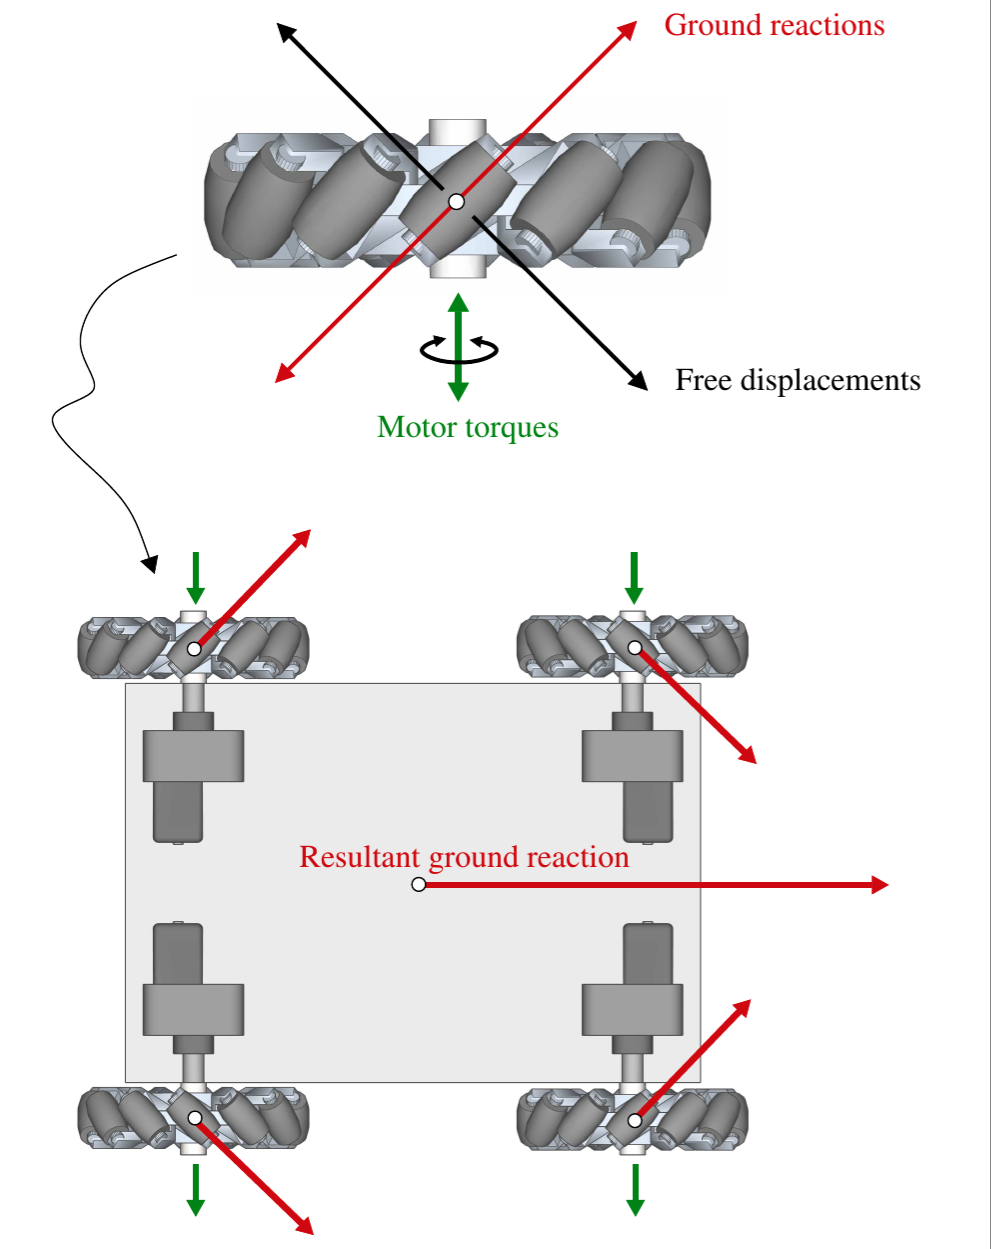
\includegraphics[width=\linewidth]{omni wheel principle.png}
            \caption{Принцип действия колеса Mecanum}
        \end{figure}
        \column{0.45\textwidth}
        \small
        Свободно вращающиеся ролики под углом $\pm 45\degree$ создают
        составляющие реакции опоры в обоих направлениях.
        \medskip

        Четыре колеса дают \textbf{голономное} перемещение в плоскости:
        свободный выбор $v_x$, $v_y$ и $\omega$ независимо.
        \medskip

        Прямая кинематика связывает скорости корпуса и угловые скорости
        колёс через $r$, $L$, $l$.
    \end{columns}
\end{frame}

%% =========================================================================
\section{MPPI и функция потерь}

\begin{frame}{Принцип MPPI}
    На каждом такте контроллер генерирует $M$ возмущённых траекторий и
    обновляет номинальное управление взвешенным средним.
    \medskip

    \[
    \boldsymbol{\epsilon}^{(m)}_{j} \sim \mathcal{N}(0,\Sigma),\quad
    \mathbf{u}^{(m)}_{k+j} = \bar{\mathbf{u}}_{k+j} + \boldsymbol{\epsilon}^{(m)}_{j},
    \]
    \[
    S^{(m)} = \sum_{j=0}^{N-1} \ell\bigl(\mathbf{x}^{(m)}_{k+j},\mathbf{u}^{(m)}_{k+j}\bigr) + \ell_f,
    \quad
    w^{(m)} = \frac{e^{-S^{(m)}/\lambda}}{\sum_q e^{-S^{(q)}/\lambda}},
    \]
    \[
    \bar{\mathbf{u}}^{\text{new}}_{k+j} =
    \bar{\mathbf{u}}_{k+j} + \sum_{m=1}^{M} w^{(m)}\,\boldsymbol{\epsilon}^{(m)}_{j}.
    \]

    \medskip
    \footnotesize
    Преимущества для задачи: произвольные негладкие штрафы (включая
    costmap), естественная параллелизация по траекториям,
    устойчивость к локальным минимумам.
\end{frame}

\begin{frame}{Составная функция потерь}
    \[
    \ell_k =
    w_d\,(e^{d}_{k})^{2}
    + w_{\phi}\,(e^{\phi}_{k})^{2}
    + w_{u}\,\|\mathbf{u}_k\|_2^{2}
    + w_{\Delta u}\,\|\mathbf{u}_k - \mathbf{u}_{k-1}\|_2^{2}
    \]
    \[
    + w_{\text{obs}}\,\Psi_{\text{obs},k}
    + w_{\text{pf}}\,\Psi_{\text{pf},k}
    + w_{\text{hold}}\,\Psi_{\text{hold},k}.
    \]
    \medskip
    \footnotesize
    \begin{itemize}
        \item $e^{d}_k$~--- отклонение от целевой дистанции $d^{\star}$;
        \item $e^{\phi}_k$~--- отклонение от азимута на цель в кадре
              камеры (центрирование);
        \item $\Psi_{\text{obs},k}$~--- изотропный барьер по
              расстоянию до препятствий
              ($d_{i,k} \to d_{\text{safe}}$);
        \item $\Psi_{\text{pf},k}$~--- направленный штраф поля
              препятствий (см.\ след.\ слайд);
        \item $\Psi_{\text{hold},k} = (1-\nu_k)\,\|\mathbf{u}_k\|_2^{2}$~---
              остановка при потере цели.
    \end{itemize}
\end{frame}

\begin{frame}{Направленный штраф поля препятствий $\Psi_{\text{pf},k}$}
    Пусть $c(x,y)\!\in\![0,1]$~--- нормированный costmap,
    $\tilde{d}(c)$~--- восстановленное по инфляционной модели
    расстояние до препятствия. Тогда
    \[
    \hat{\mathbf{f}}_k = -\frac{\nabla c(\mathbf{p}_k)}{\|\nabla c(\mathbf{p}_k)\|_2},
    \quad
    \rho_k = \max\bigl(0,\, d^{\star}_{\text{pf}} - \tilde{d}(c(\mathbf{p}_k))\bigr),
    \]
    \[
    \sigma_k = \max\bigl(0,\, -\langle \hat{\mathbf{v}}_k, \hat{\mathbf{f}}_k\rangle\bigr)\,(1+\rho_k),
    \]
    \[
    \Psi_{\text{pf},k}
    = \mathbf{1}\!\bigl[c(\mathbf{p}_k)\ge c_{\text{act}}\bigr]\,
    \bigl(w_{\rho}\,\rho_k + w_{\sigma}\,\sigma_k\bigr).
    \]
    \medskip
    Активация по порогу $c_{\text{act}}$ и отключение в радиусе
    $d_{\text{ng}}$ от цели.
\end{frame}

\begin{frame}{Декомпозиция на критики Nav2/MPPI}
    \scriptsize
    \begin{tabularx}{\textwidth}{l X}
        \toprule
        \textbf{Слагаемое функции потерь} & \textbf{Критик(и)} \\
        \midrule
        Ограничения скоростей $|v|\le v^{\max}$
        & \texttt{ConstraintCritic} \\
        $\Psi_{\text{obs},k}$ (изотропный)
        & \texttt{CostCritic}, \texttt{ObstaclesCritic} \\
        $\Psi_{\text{pf},k}$ (направленный)
        & \texttt{PotentialFieldCritic} \emph{(реализован в ВКР)} \\
        $w_{\phi}(e^{\phi}_k)^2$ (центрирование цели)
        & \texttt{TargetCameraCritic} \emph{(реализован в ВКР)} \\
        Терминальные слагаемые
        & \texttt{GoalCritic} \\
        Удержание у пути планировщика
        & \texttt{PathAlignCritic}, \texttt{PathFollowCritic} \\
        Подавление избыточного вращения
        & \texttt{TwirlingCritic} \\
        \bottomrule
    \end{tabularx}
    \medskip

    \footnotesize
    Каждый критик~--- независимый модуль; параметры настраиваются
    отдельно (\texttt{config/omni\_nav2\_params.yaml}).
\end{frame}

\begin{frame}{Сцена симуляции}
    \begin{columns}[T,onlytextwidth]
        \column{0.5\textwidth}
        \begin{figure}
            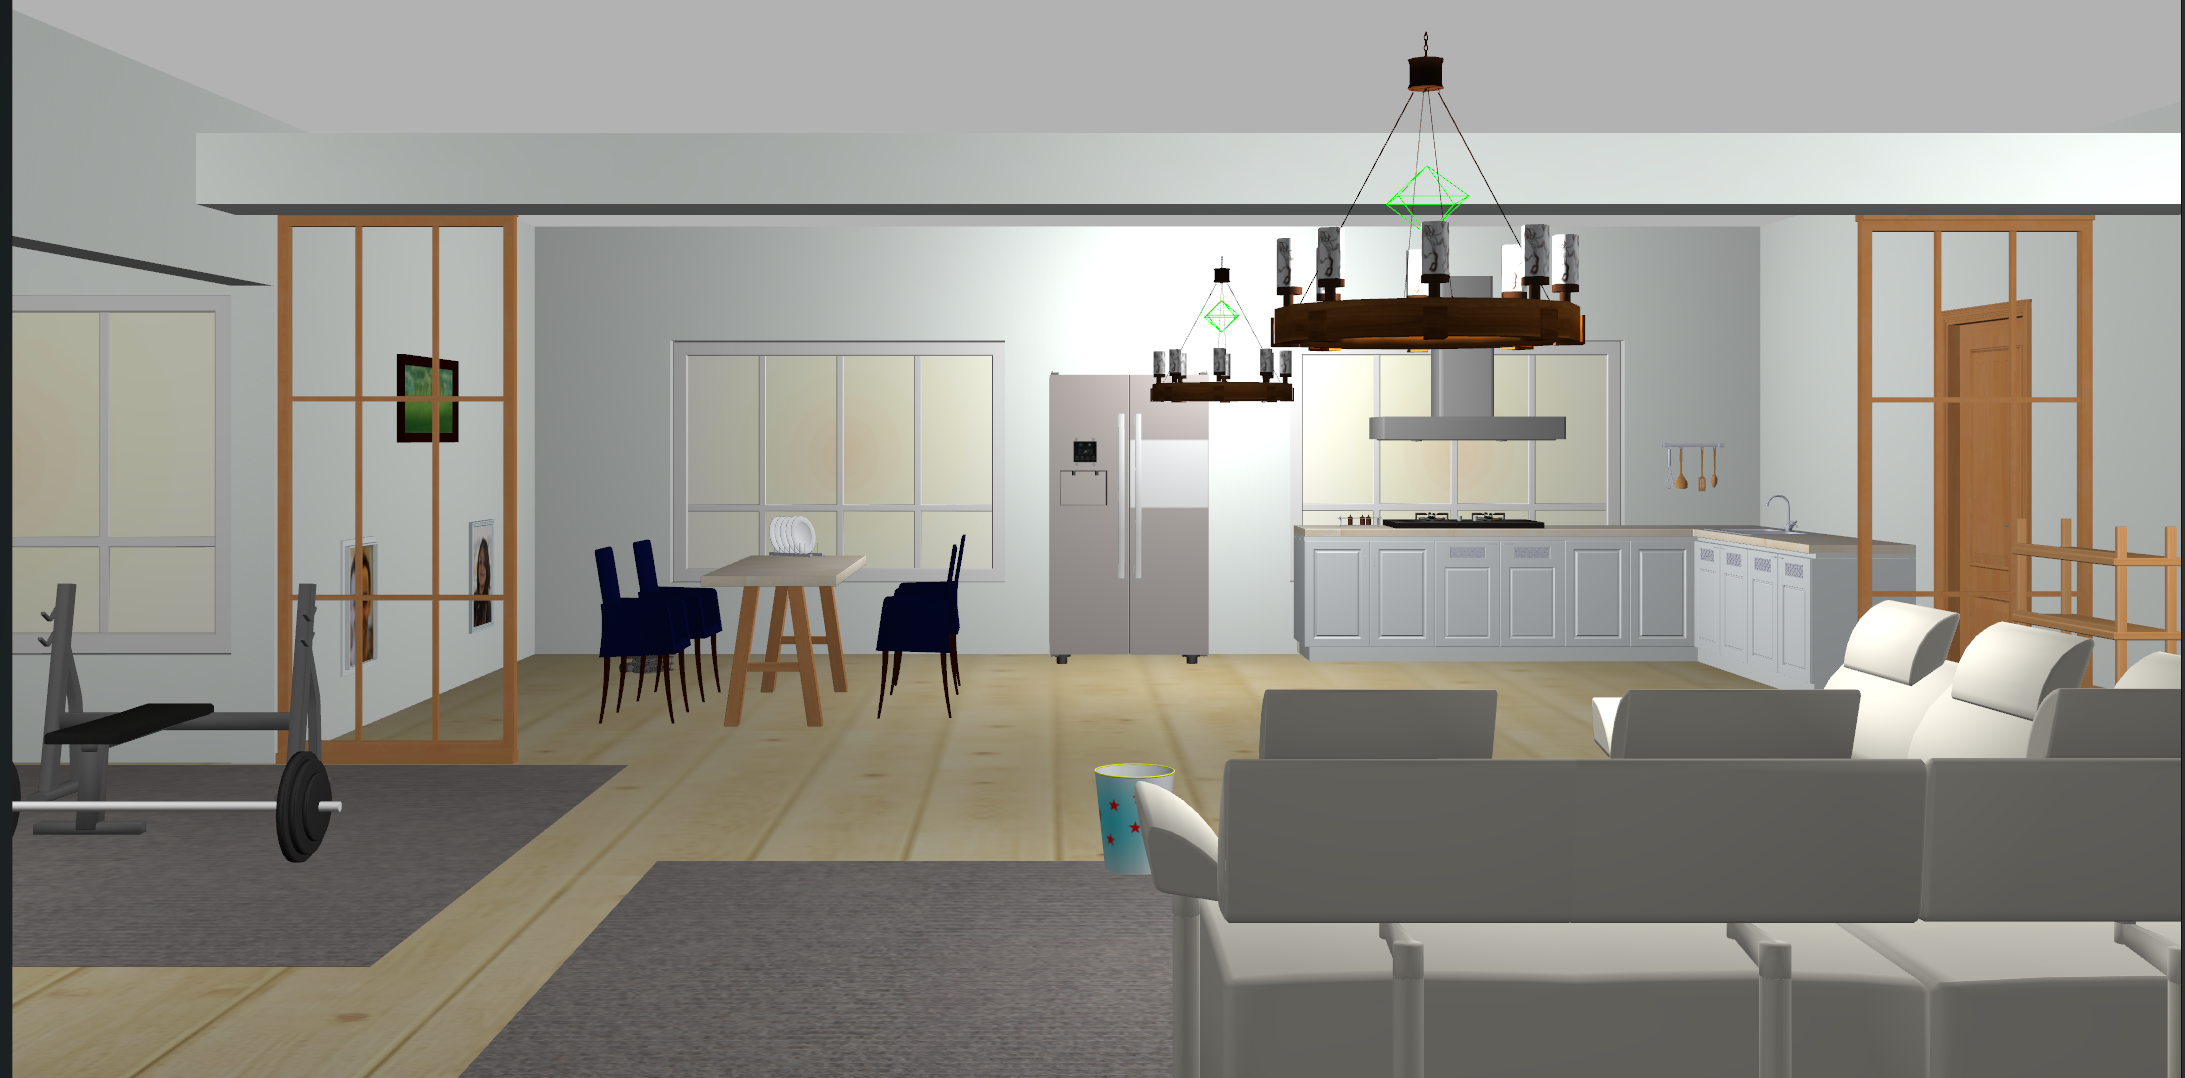
\includegraphics[width=\linewidth]{house.png}
            \caption{Сцена симуляции квартиры}
        \end{figure}
        \column{0.5\textwidth}
        \begin{figure}
            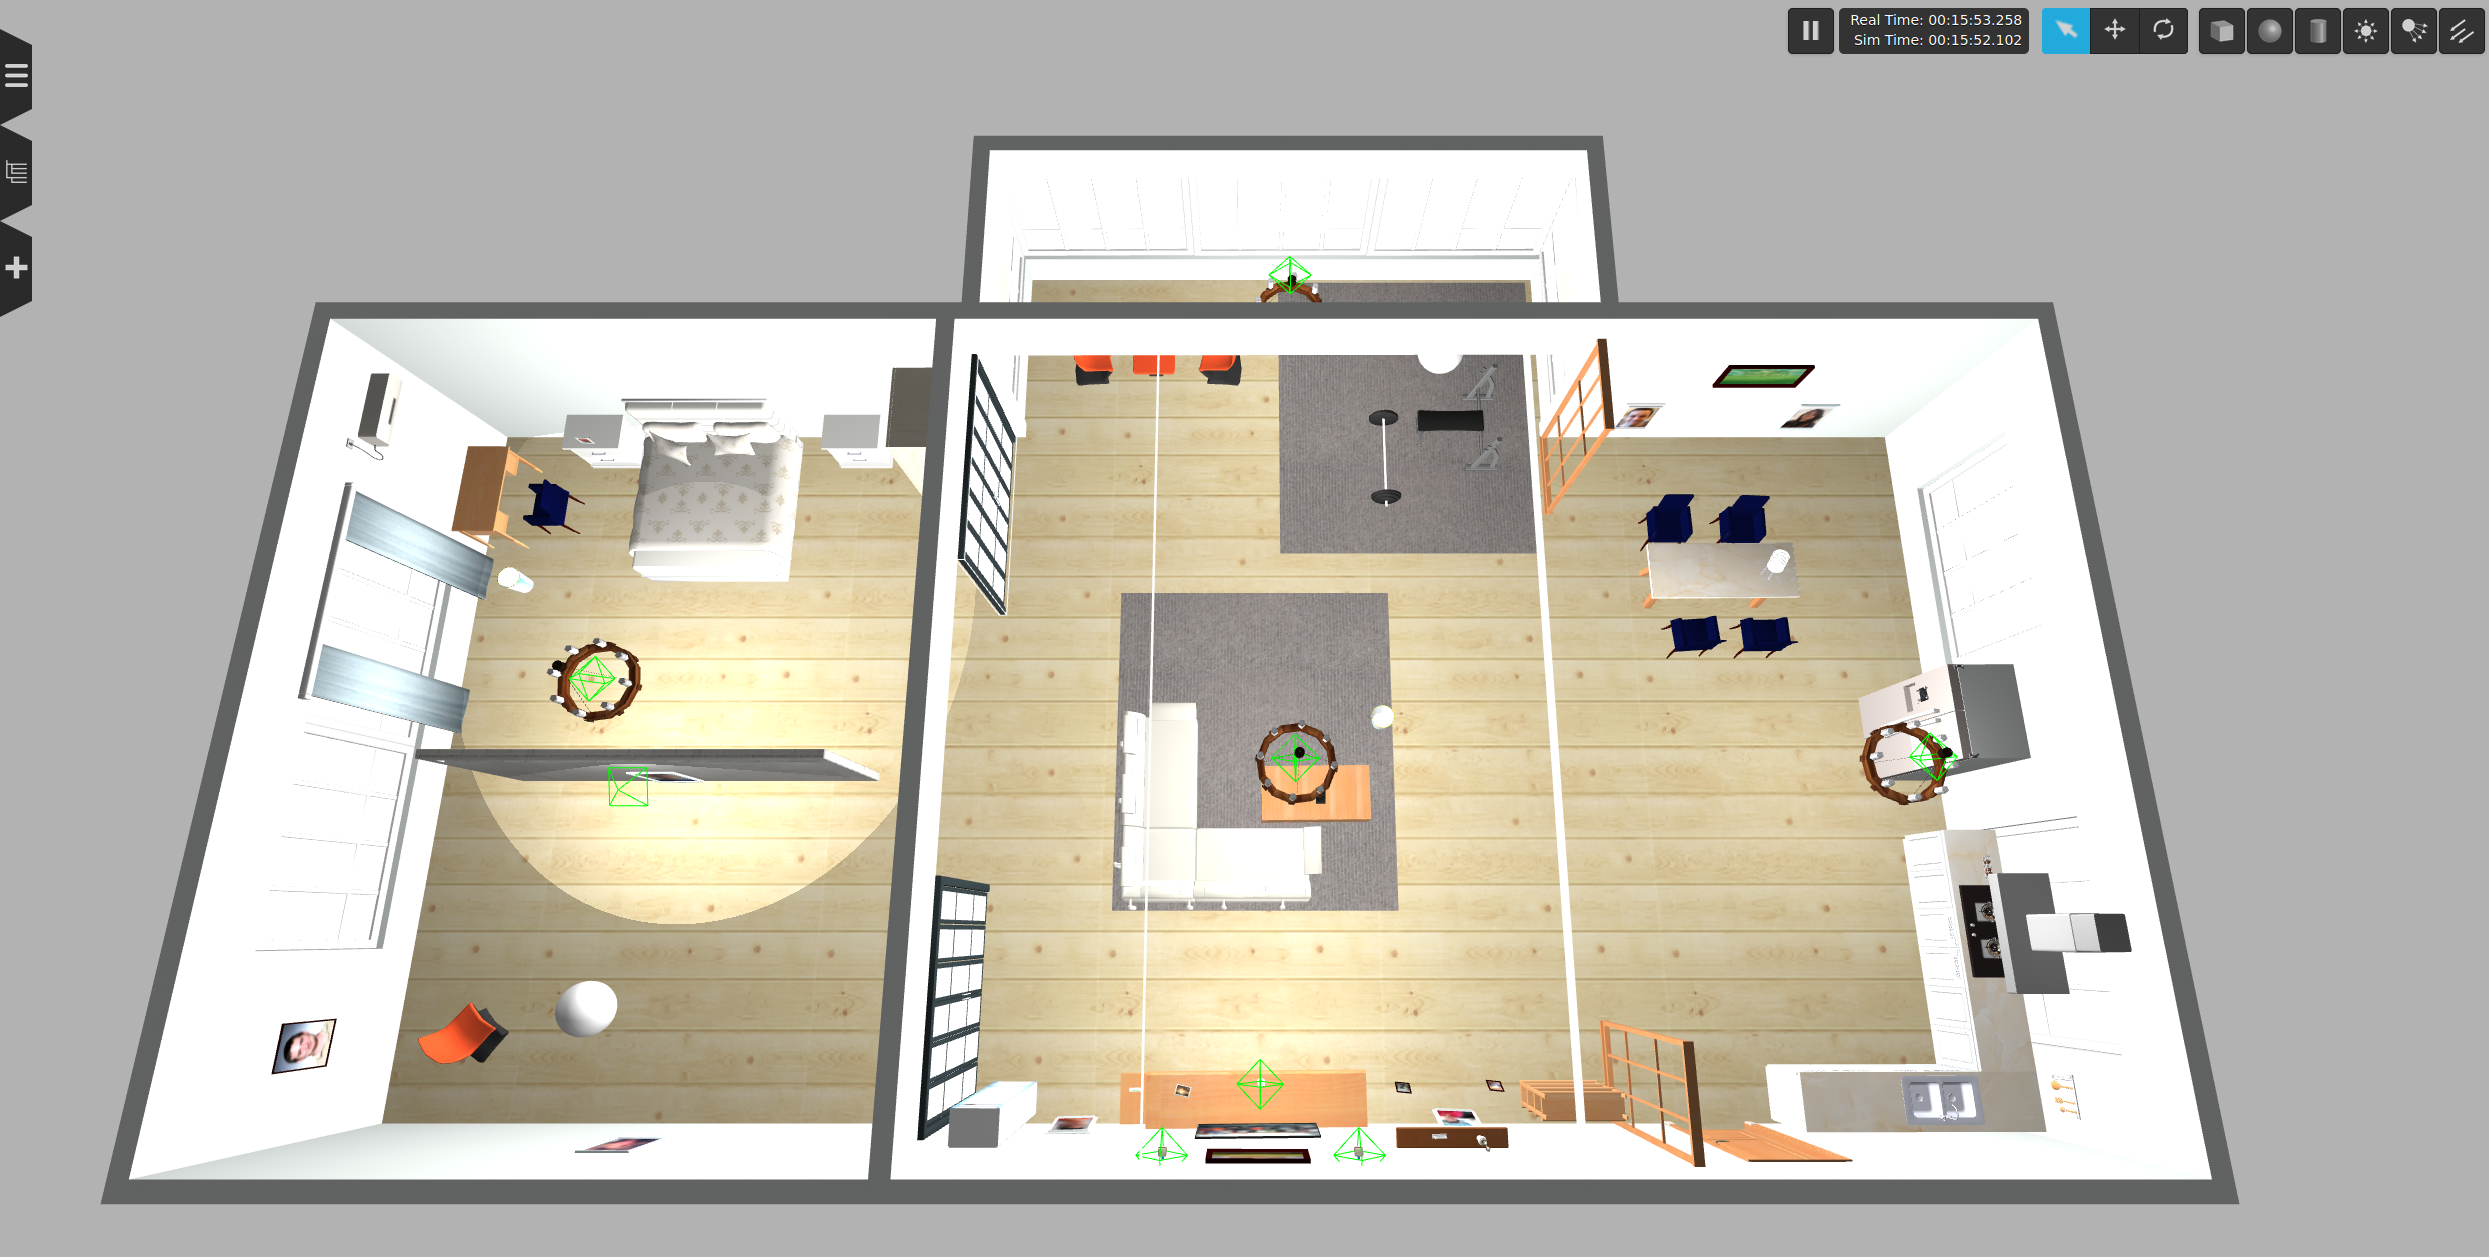
\includegraphics[width=\linewidth]{house_up.png}
            \caption{Сцена симуляции (вид сверху)}
        \end{figure}
    \end{columns}
    \medskip

    \footnotesize
    Стены, мебель и свободное пространство, достаточное для
    маневрирования; цель (синий цилиндр) и подвижные цилиндрические
    препятствия со случайными скоростями~--- пакет
    \texttt{apartment\_sim}.
\end{frame}

\begin{frame}{Рабочая сцена системы}
    \begin{figure}
        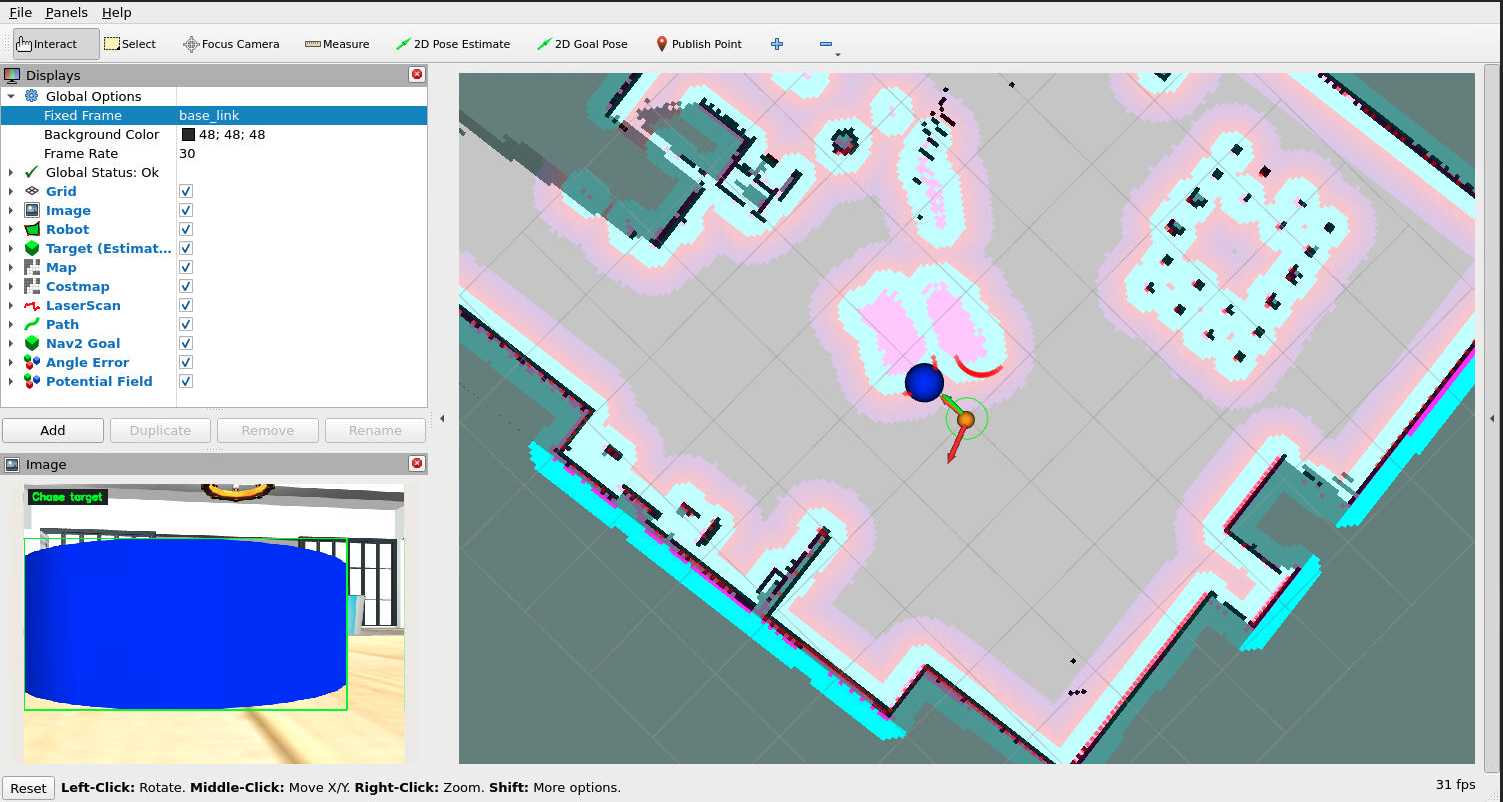
\includegraphics[width=0.80\linewidth]{rviz screenshot.png}
        \caption{RViz: карта, costmap, лидар, путь, маркер цели,
        кадр камеры с индикатором видимости}
    \end{figure}
\end{frame}

%% =========================================================================
\section{Эксперименты}
\begin{frame}{Один запуск: режимы сопровождения}
    \begin{figure}
        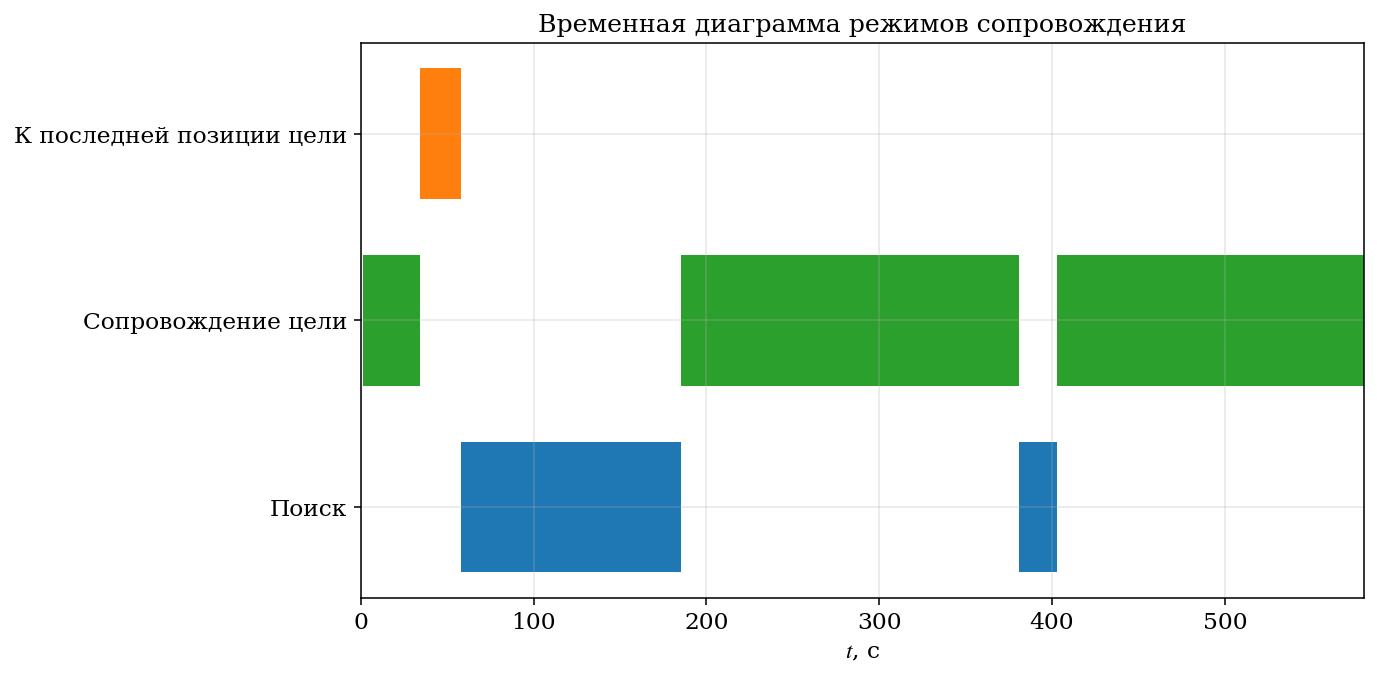
\includegraphics[width=0.9\linewidth]{exp_mode_timeline_run.png}
        \caption{Временная диаграмма режимов сопровождения}
    \end{figure}
    \footnotesize
    Доминирует режим \textit{Сопровождение цели}; кратковременные
    переходы в \textit{Поиск} соответствуют эпизодам потери цели.
\end{frame}

\begin{frame}{Один запуск: видимость цели}
    \begin{figure}
        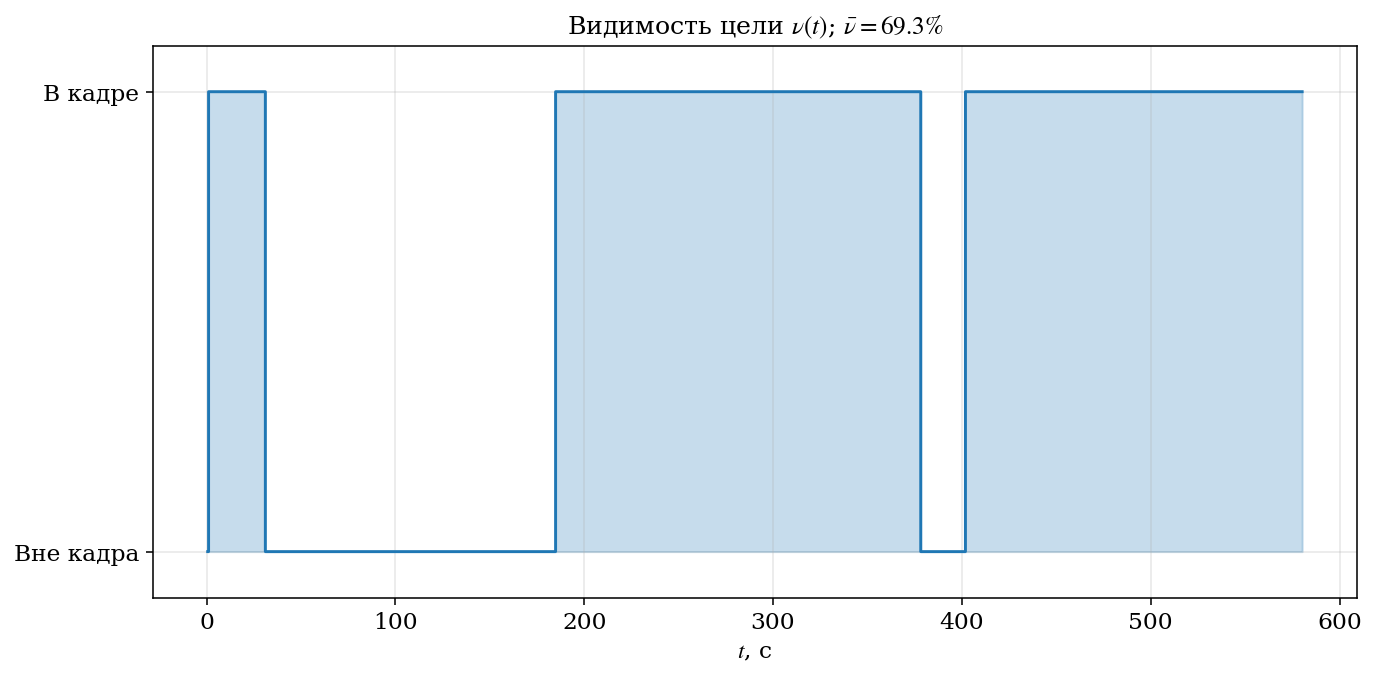
\includegraphics[width=0.9\linewidth]{exp_visibility_run.png}
        \caption{Видимость цели $\nu(t)$ ($\bar{\nu}\approx 69{,}3\%$)}
    \end{figure}
    \footnotesize
    Падения соответствуют моментам, когда подвижное препятствие
    закрывает цель; совпадают с переключением в режим
    \textit{Поиск}.
\end{frame}

\begin{frame}{Один запуск: безопасность}
    \begin{figure}
        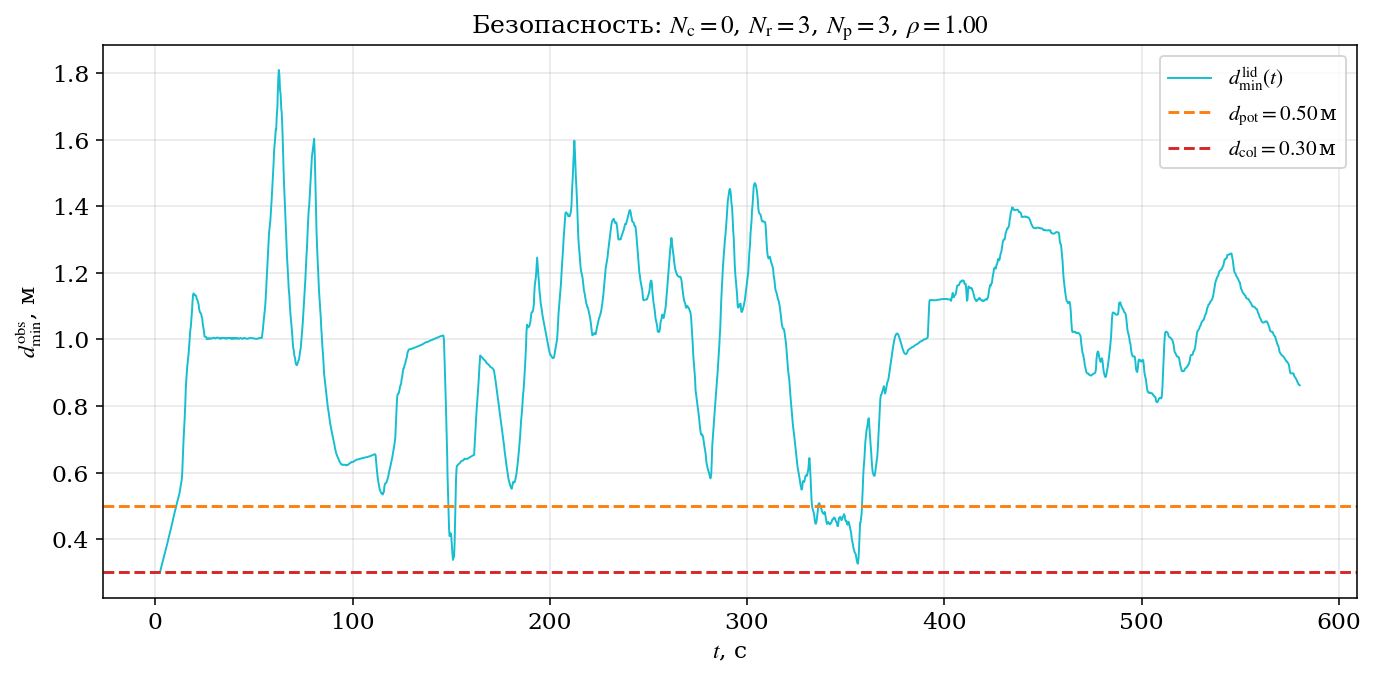
\includegraphics[width=0.9\linewidth]{exp_safety_distance_run.png}
        \caption{$d^{\text{lid}}_{\min}(t)$ с порогами $d_{\text{pot}}$ и $d_{\text{col}}$;
        $N_{\text{c}}=0$, $N_{\text{r}}=3$, $N_{\text{p}}=3$, $\rho=1{,}00$}
    \end{figure}
    \footnotesize
    Заходы в зону риска есть, но фактических контактов нет~---
    совместный эффект $\Psi_{\text{obs}}$ и $\Psi_{\text{pf}}$.
\end{frame}

\begin{frame}{Один запуск: плавность управления}
    \begin{figure}
        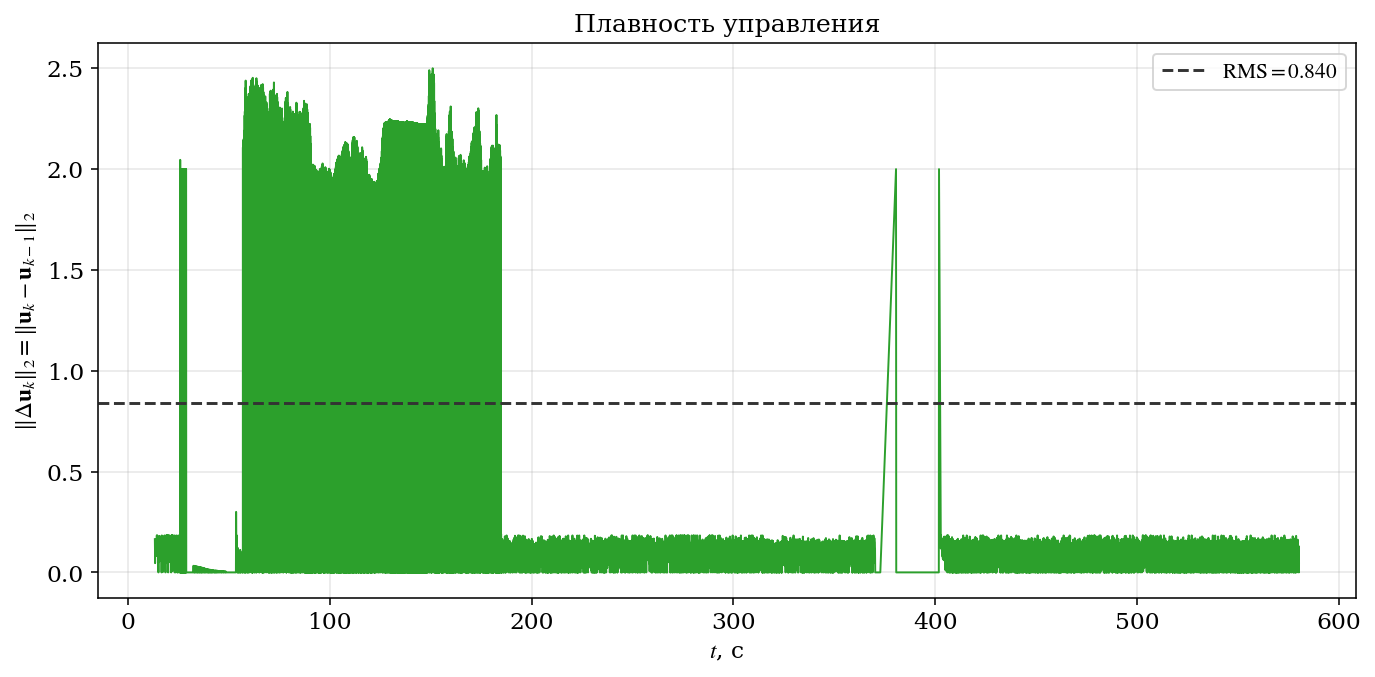
\includegraphics[width=0.9\linewidth]{exp_control_smoothness_run.png}
        \caption{$\|\Delta\mathbf{u}_k\|_2$ и его $\mathrm{RMS}$}
    \end{figure}
    \footnotesize
    Повышенные значения соответствуют моментам маневрирования и
    переключений режимов; на длинных участках сопровождения
    приращения близки к нулю.
\end{frame}

\begin{frame}{Серия из 40 запусков: режимы}
    \begin{figure}
        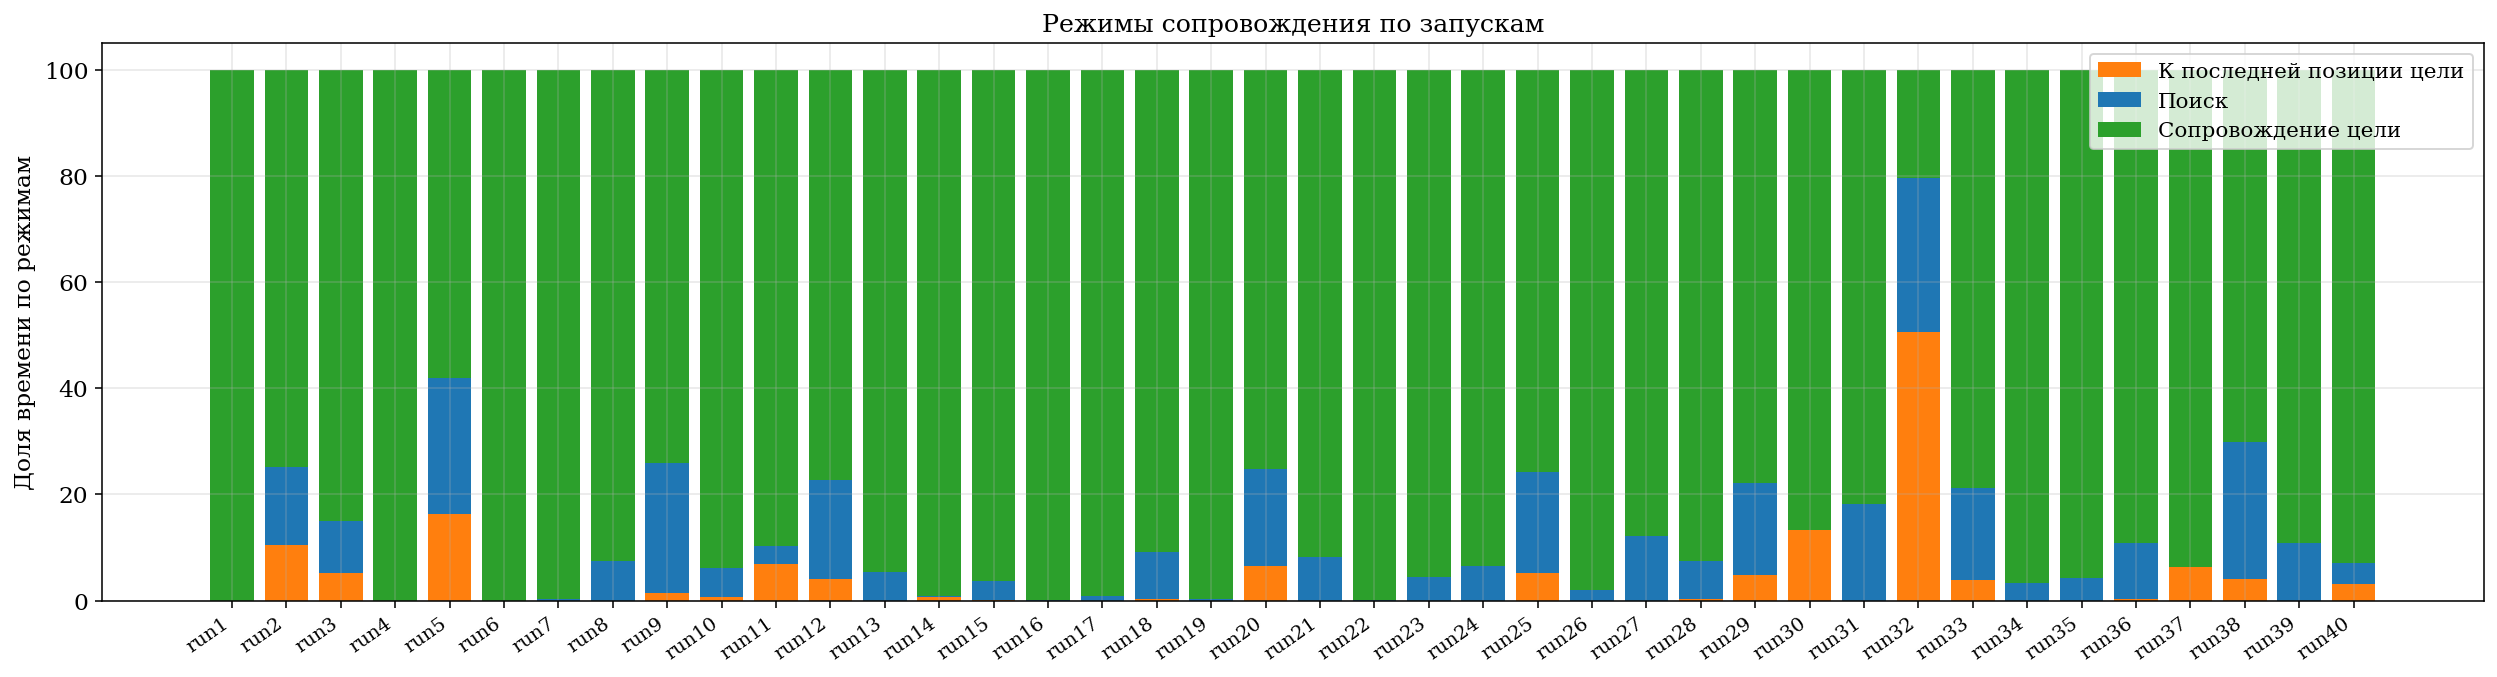
\includegraphics[width=1.0\linewidth]{exp_all_mode_shares.png}
        \caption{Доли времени по режимам сопровождения по запускам}
    \end{figure}
    \footnotesize
    Во всех запусках доминирует режим \textit{Сопровождение цели};
    в большинстве запусков совокупная доля \textit{Поиска} и
    \textit{К~последней позиции цели} меньше 25\%.
\end{frame}

\begin{frame}{Серия из 40 запусков: видимость}
    \begin{figure}
        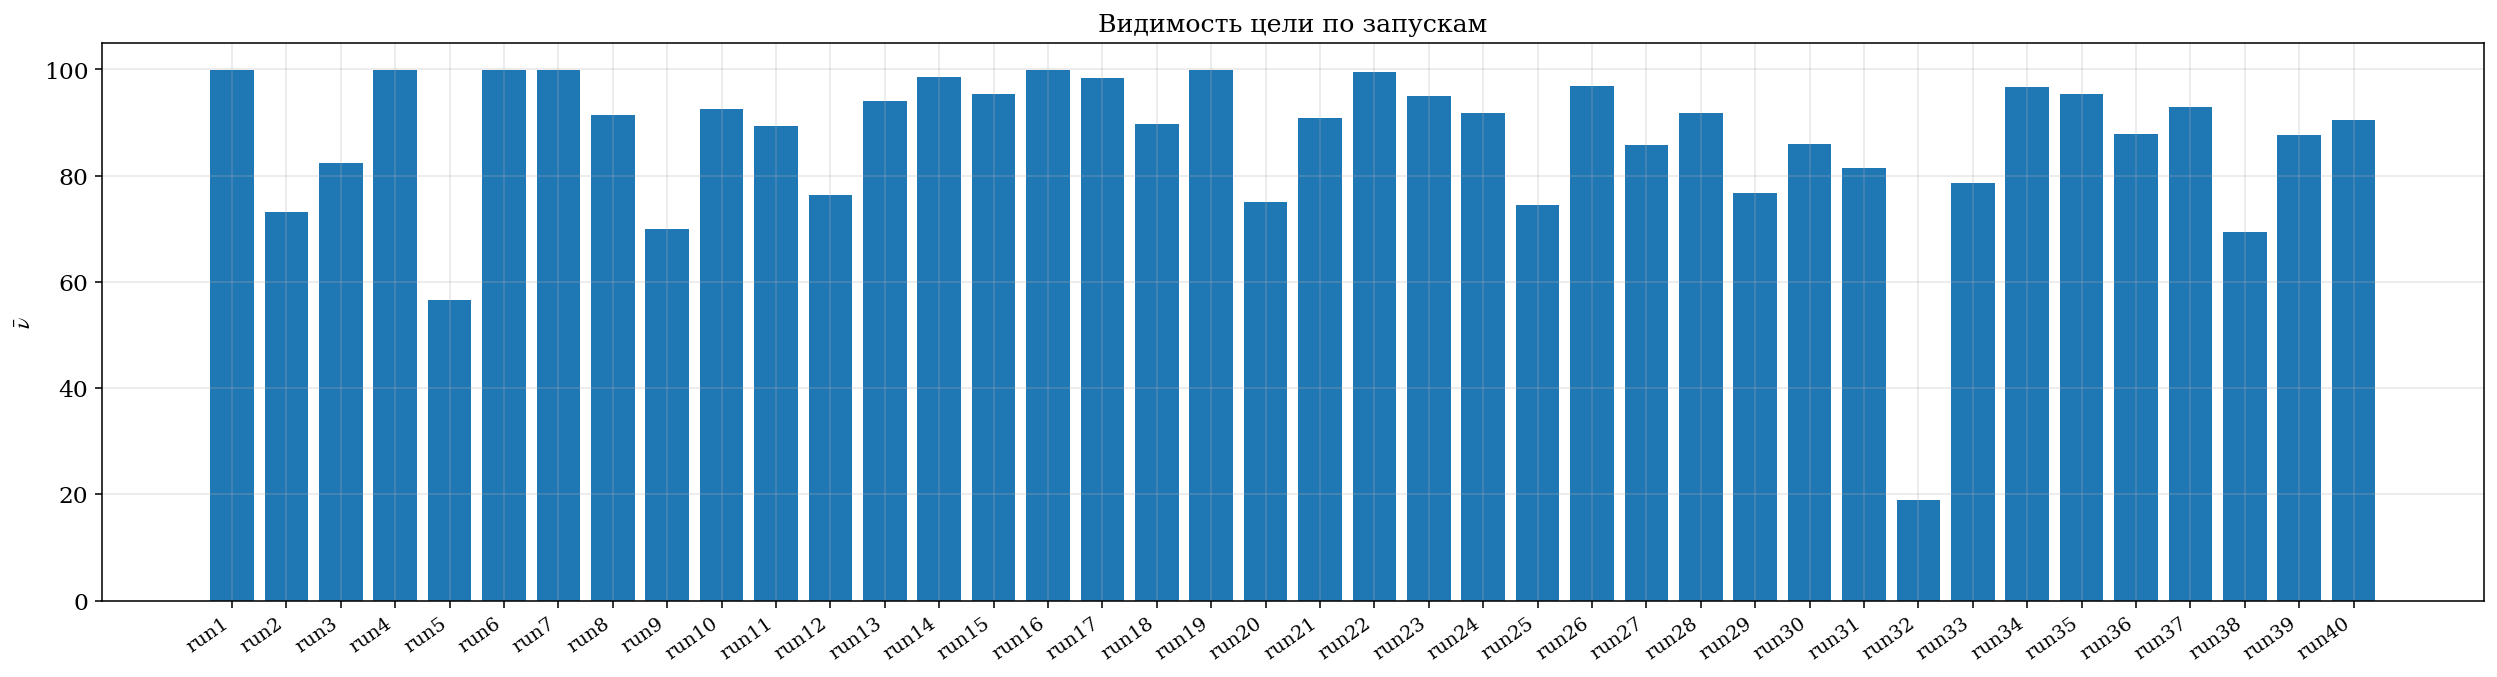
\includegraphics[width=1.0\linewidth]{exp_all_visibility.png}
        \caption{Доля времени видимости цели $\bar{\nu}$ по запускам}
    \end{figure}
    \footnotesize
    В большинстве запусков $\bar{\nu} > 80\%$; единичные просадки
    соответствуют сценариям с систематическим закрытием цели
    подвижными препятствиями.
\end{frame}

\begin{frame}{Серия из 40 запусков: безопасность}
    \begin{figure}
        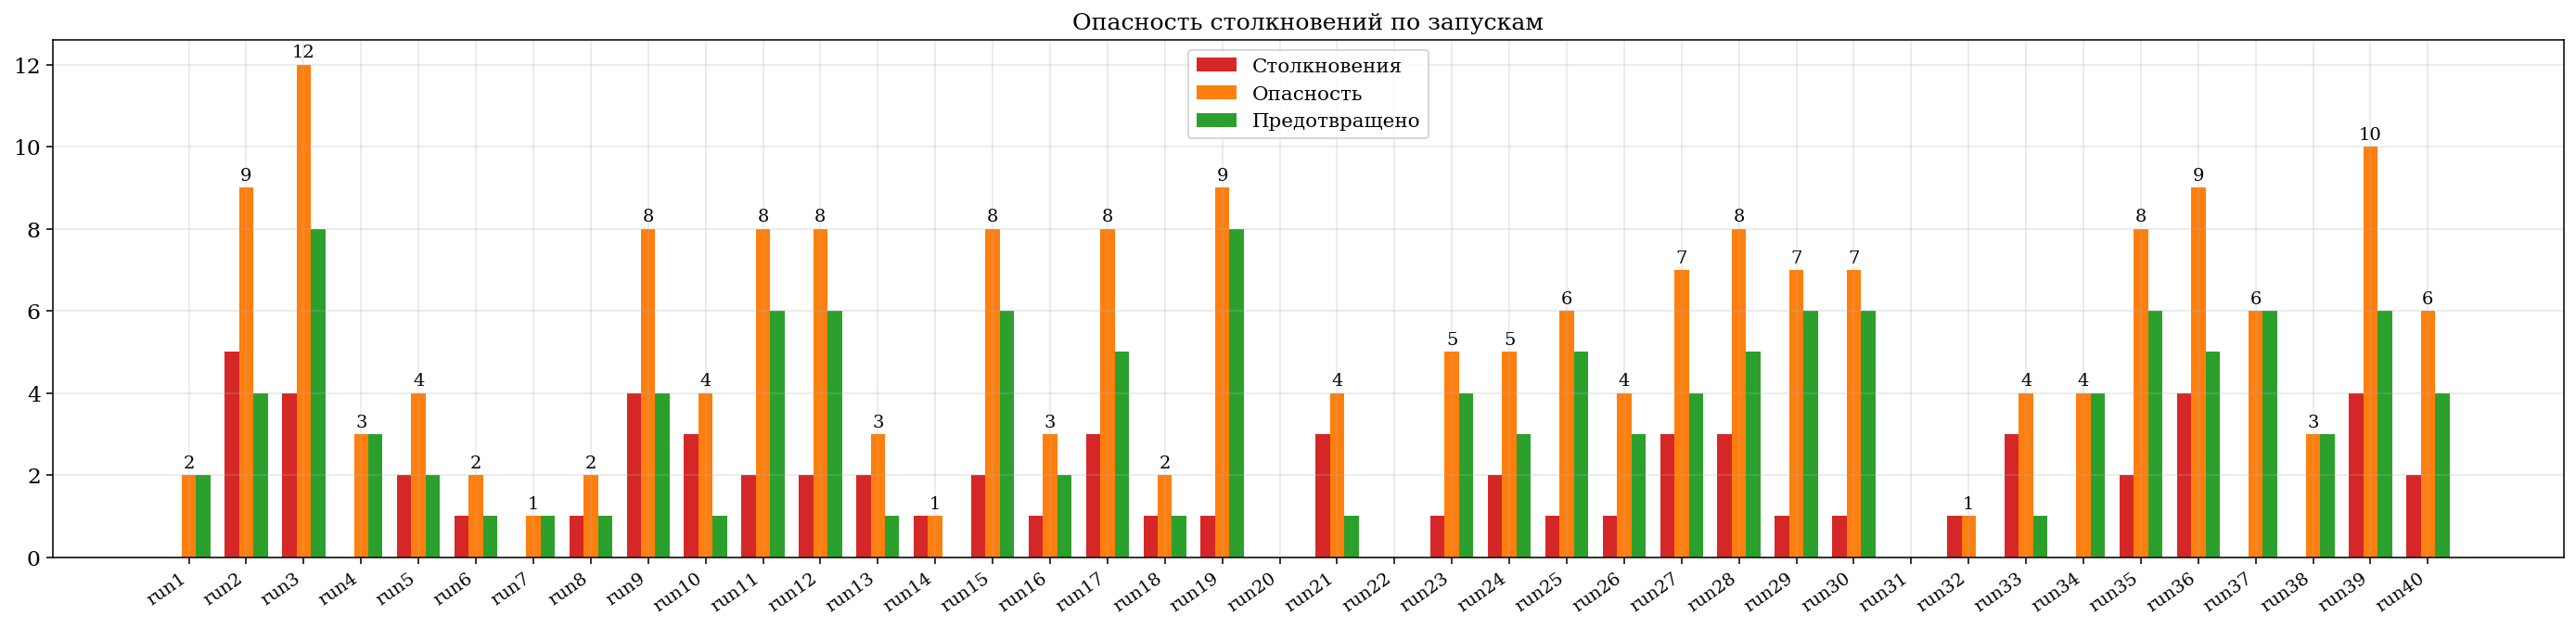
\includegraphics[width=1.0\linewidth]{exp_all_safety_events.png}
        \caption{Столкновения $N_{\text{c}}$, заходы в зону риска
        $N_{\text{r}}$, предотвращённые контакты $N_{\text{p}}$}
    \end{figure}
    \footnotesize
\end{frame}

\begin{frame}{Серия из 40 запусков: плавность управления}
    \begin{figure}
        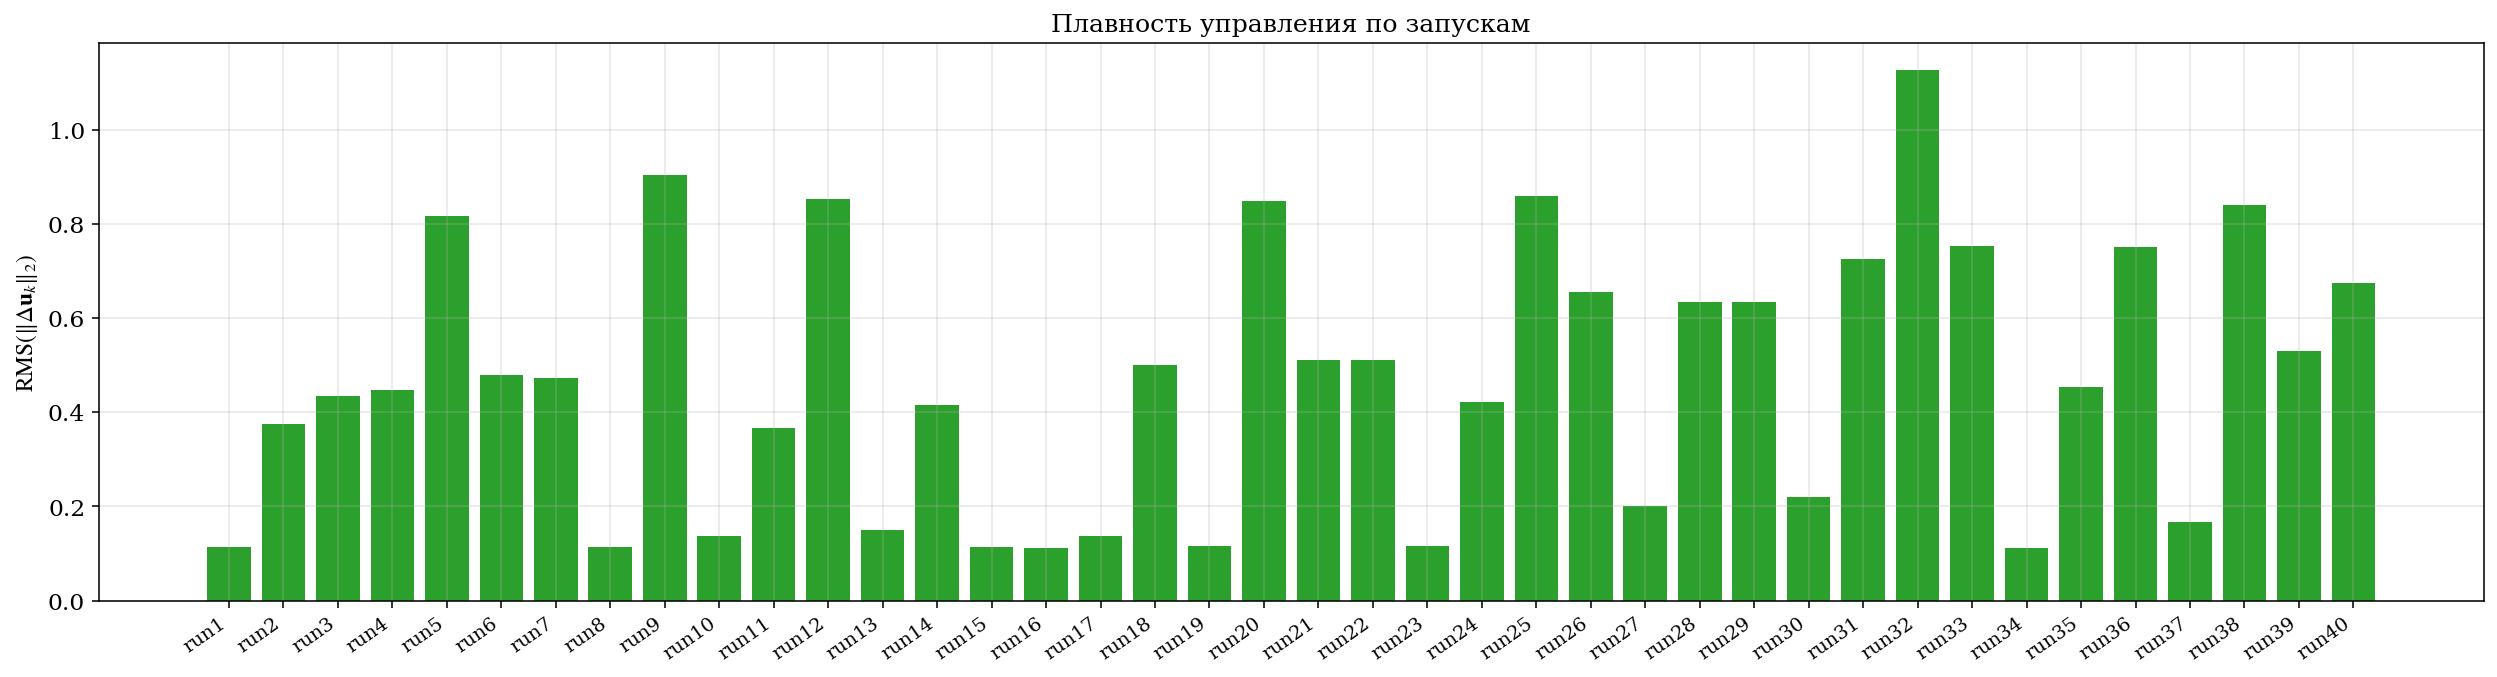
\includegraphics[width=1.0\linewidth]{exp_all_control_smoothness.png}
        \caption{$\mathrm{RMS}(\|\Delta\mathbf{u}_k\|_2)$ по запускам}
    \end{figure}
    \footnotesize
\end{frame}

%% =========================================================================
\section{Заключение}

\begin{frame}{Основные результаты}
    \footnotesize
    \begin{enumerate}
        \item Проанализированы подходы к локальному планированию и
              SLAM; обоснован выбор MPPI, \texttt{slam\_toolbox} и
              Nav2.
        \item Построена кинематическая модель омни-платформы
              Mecanum; формализована составная функция потерь, в том
              числе слагаемое $\Psi_{\text{pf},k}$.
        \item Развёрнута воспроизводимая контейнерная среда
              исполнения с автоматизацией стартовой
              последовательности и удалённым доступом к GUI.
        \item Реализованы пользовательские критики
              \texttt{TargetCameraCritic} и
              \texttt{PotentialFieldCritic} в составе
              \texttt{nav2\_mppi\_controller}.
        \item Автоматизирован сбор статистики по экспериментам; подтверждены доминирование
              режима \textit{Сопровождение цели}, высокая средняя
              видимость цели, систематическое превышение
              $N_{\text{r}}$ над $N_{\text{c}}$ и приемлемая
              плавность контура управления.
    \end{enumerate}
\end{frame}

\begin{frame}{Перспективы}
    \begin{itemize}
        \item Замена цветового детектора на детектор машинного
              обучения (YOLO-класса) для произвольного пользователя.
        \item Перенос на реальную платформу Mecanum-типа с
              переопределением весов функции потерь по данным
              полевых испытаний.
    \end{itemize}
\end{frame}

\begin{frame}[plain]
    \vfill
    \begin{center}
        {\Large\bfseries Спасибо за внимание}\\[1.5em]
        \large Готов ответить на вопросы.
    \end{center}
    \vfill
\end{frame}

\end{document}
